% \section{Markstein Flame Modelling}

% Finding the Markstein number is crucial to predicting the behaviour of flames.

% LITERATURE:
% \begin{itemize}
% \item \cite{clavin1982EffectsMolecularDiffusion} the first theoretical prediction of Markstein number from asymptotic theory
% \item \cite{matalon1982FlamesGasdynamicDiscontinuities} also predicted the same Markstein number in the same year from similar asymptotics
% \item \cite{searby1991ParametricAcousticInstability} proposes Mathieu model for secondary thermoacoustic instability. This is used to predict Markstein numbers experimentally by comparing sound frequency at the onset of parametric instability to the acoustic amplitude and comparing this data to theoretical predictions at different Markstein numbers. The disturbance wavenumber is also proposed as a method to find this Markstein number in a similar way.
% \item \cite{delfin2024DeterminationMethodMarkstein} measures Markstein numbers using the proposed method from \cite{searby1991ParametricAcousticInstability} by measuring disturbance wavenumbers at the onset of secondary instability and comparing them to theoretical values.
% \item \cite{day2009TurbulenceEffectsCellular} calculates Markstein numbers from simulation data for lean premixed H2-air combustion by computing JPDFs of flame speed against flame curvature. Each data point in these JPDFs is an \emph{integral tubes} (the area bounded by 3 or more integral curves, in 3D) of $\vec{\nabla} c$ for $c$ the reactant progress variable with values taken at $c=0.98$, representing the position of the flame.
% \item \cite{howarth2022EmpiricalCharacteristicScaling} and \cite{howarth2023ThermodiffusivelyunstableLeanPremixed} follow the same method as \cite{day2009TurbulenceEffectsCellular}, but incorporates the strain term to the right-hand side calculation, uses $c=0.9$. Care is taken to ensure that the chosen flame surface is representative of the flame. They also evaluate individual Markstein numbers for the curvature and strain term on the RHS, as suggested in \cite{clavin2011CurvedStretchedFlames} (TALK ABOUT THIS PAPER ABOVE??).
% \item \cite{davis2002MarksteinNumbersCounterflow} compares markstein numbers calculated from unburnt and burnt velocity values. (NEED TO READ??)
% \item Al Sarraf ??
% \item Aldredge ??
% \end{itemize}








\section{Combustion Instabilities}

% Thermoacoustics background - can cover what was in 1YR

\subsection{G-Equation Model}




\subsection{Primary vs. Secondary Thermoacoustic Instabilities}


\begin{figure}[t]
\centering
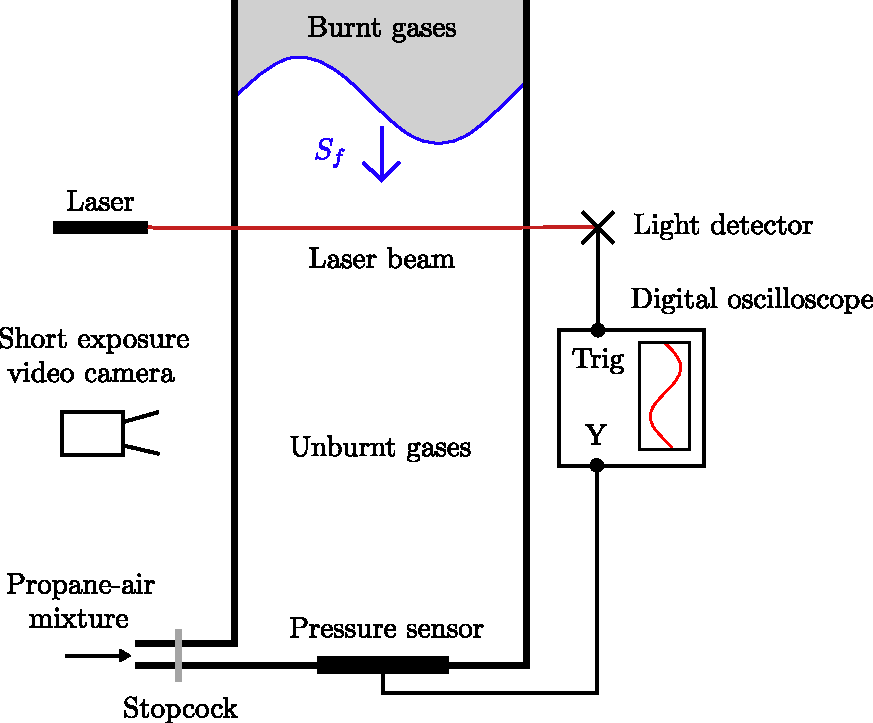
\includegraphics[scale=0.6]{assets/imgs/Searby-92.pdf}
\caption{SEARBY EXPERIMENT}
\label{fig:searby-experiment}
\end{figure}

\begin{figure}[t]
\centering
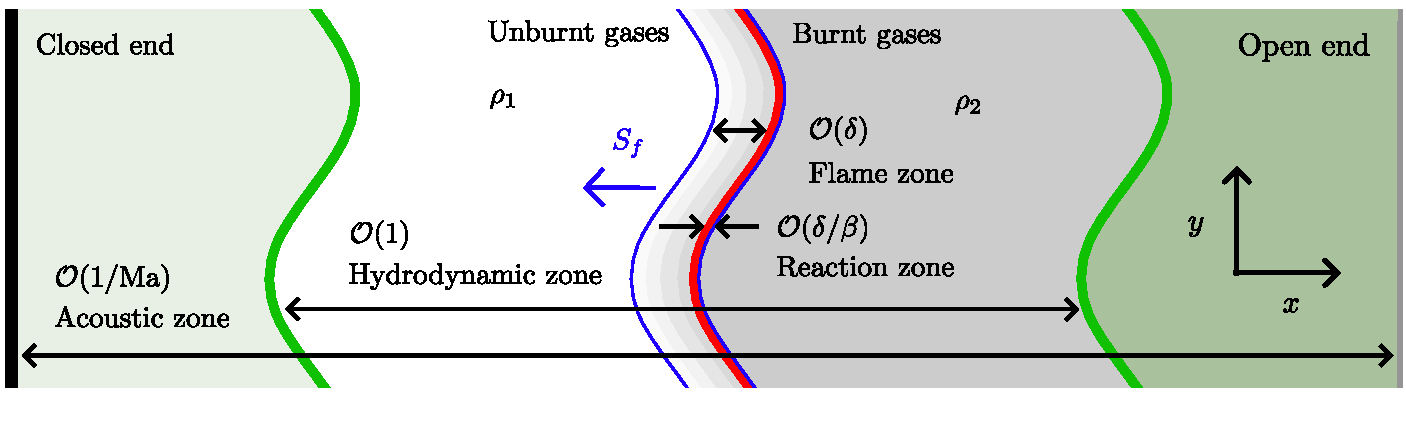
\includegraphics[scale=0.6]{assets/imgs/AW-flame.pdf}
\caption{AW FLAME}
\label{fig:AW-flame}
\end{figure}
    
        


\subsection{Low-Order Thermoacoustic Modelling}

% n-tau models


\subsection{Intrinsic Thermoacoustic Feedback}

% ITA modes!




\section{Numerical Combustion Simulation}

\cite{orszag1970AnalyticalTheoriesTurbulence, domingo2023RecentDevelopmentsDNS, chen2011PetascaleDirectNumerical, yang2015LargeeddySimulationPresent, veynante2002TurbulentCombustionModeling, moin1998DirectNumericalSimulation, tennekes1972FirstCourseTurbulence}

% The most blunt way to simulate a fluid system would be one where you try to accurately simulate every detail involved in the fluid.
% This idea was first studied by Orszag, where he defines direct numerical simulations as a numerical simulation with enough grid points to full resolve the smallest physical phenomena in the system
% Originally, Orszag studied this in the context of turbulent flows. In turbulent flows, we have vortices not only on the order of the typical flow length scale $L$, called the integral length scale, but also of sizes all the way down to the smallest turbulence scale known as the kolmogorov microscale, where the rate at which viscous dissipation effects dampen vortices far exceeds the inertial forces of the vortex.
% The size of this kolmogorov length scale is determined by the turbulent reynolds number and the integral scale with the relationship

% An alternative method that is widely used is LES and involves using models to estimate the transfer of energy at the smallest scale rather than fully simulating them [cite les review: Yang 2015]
% DNS for turbulent combustion are reviewed in \textbf{Domingo and Vervisch 2023} (with connection to LES) and \textbf{Chen 2011}.

% For small-scale, low-speed methan-air and hydrogen-air combustion, the flows we look at have similar properties to air, so are not very viscous meaning the smallest scale vortices in a fully developed turbulent may be ~...?
% But the turbulence usually isn't our biggest worry, since we also have the thin region that the reaction is taking place to resolve, usually only 300 {\textmu}m which is resolved with ~15 nodes in a high order code
% Regardless, when performing DNS careful consideration must be made to use ample sample points

% ?? DNS with simple transport / chemical schemes?

\subsection{High-Order Discretisation}




\subsection{Characteristic Boundaries}

\cite{thompson1987TimeDependentBoundary, thompson1990TimeDependentBoundaryConditions, poinsot1992BoundaryConditionsDirect, poinsot2005TheoreticalNumericalCombustion, sutherland2003ImprovedBoundaryConditions}

% [Thompson 1987, 1990, Poinsot and Lele 1992, Sutherland and Kennedy 2003, Poinsot and Veynante 2005]


% Many types of boundary conditions may be chosen for combustion schemes:
%% Periodic are very simple to enforce numerically so require no elaboration
%% No-slip or slip wall conditions
%% isothermal or adiabatic walls
%% acoustically reflecting or non-reflecting walls or inflow / outflow
%% In the case of inflow / outflow many more cases

% In most of these cases, we can use the formalism called characteristic boundary conditions (characteristic BCs)




% The simplest boundary conditions, i.e. those with constant (Dirichlet) boundary values (p=const), usually reflect acoustic waves back toward the interior of the domain. For most situations we want to simulate, this doesn't represent the physical situation, where we would rather pretend the medium continues outside of the compuational domain. This motivates a need for boundary conditions which do not reflect acoustic waves - non-reflecting boundary conditions. The formalisms are based of characteristic waves entering / leaving the domain

% Fixed velocity inlets give full reflections, so cannot be used in a non-reflecting case.

% Immersed boundary methods are also an option and open up possibilities for boundaries not restricted specific node placement, especially for moving boundaries. But as detailed in King 2022, these a largely restricted to lower order accuracy at these boundaries (cite, and for what reason?).



\subsection{Impedance Boundaries}






\section{Mesh-free Methods}

\cite{monaghan1992SmoothedParticleHydrodynamics, vacondio2021GrandChallengesSmoothed}


\begin{figure}[t]
\centering
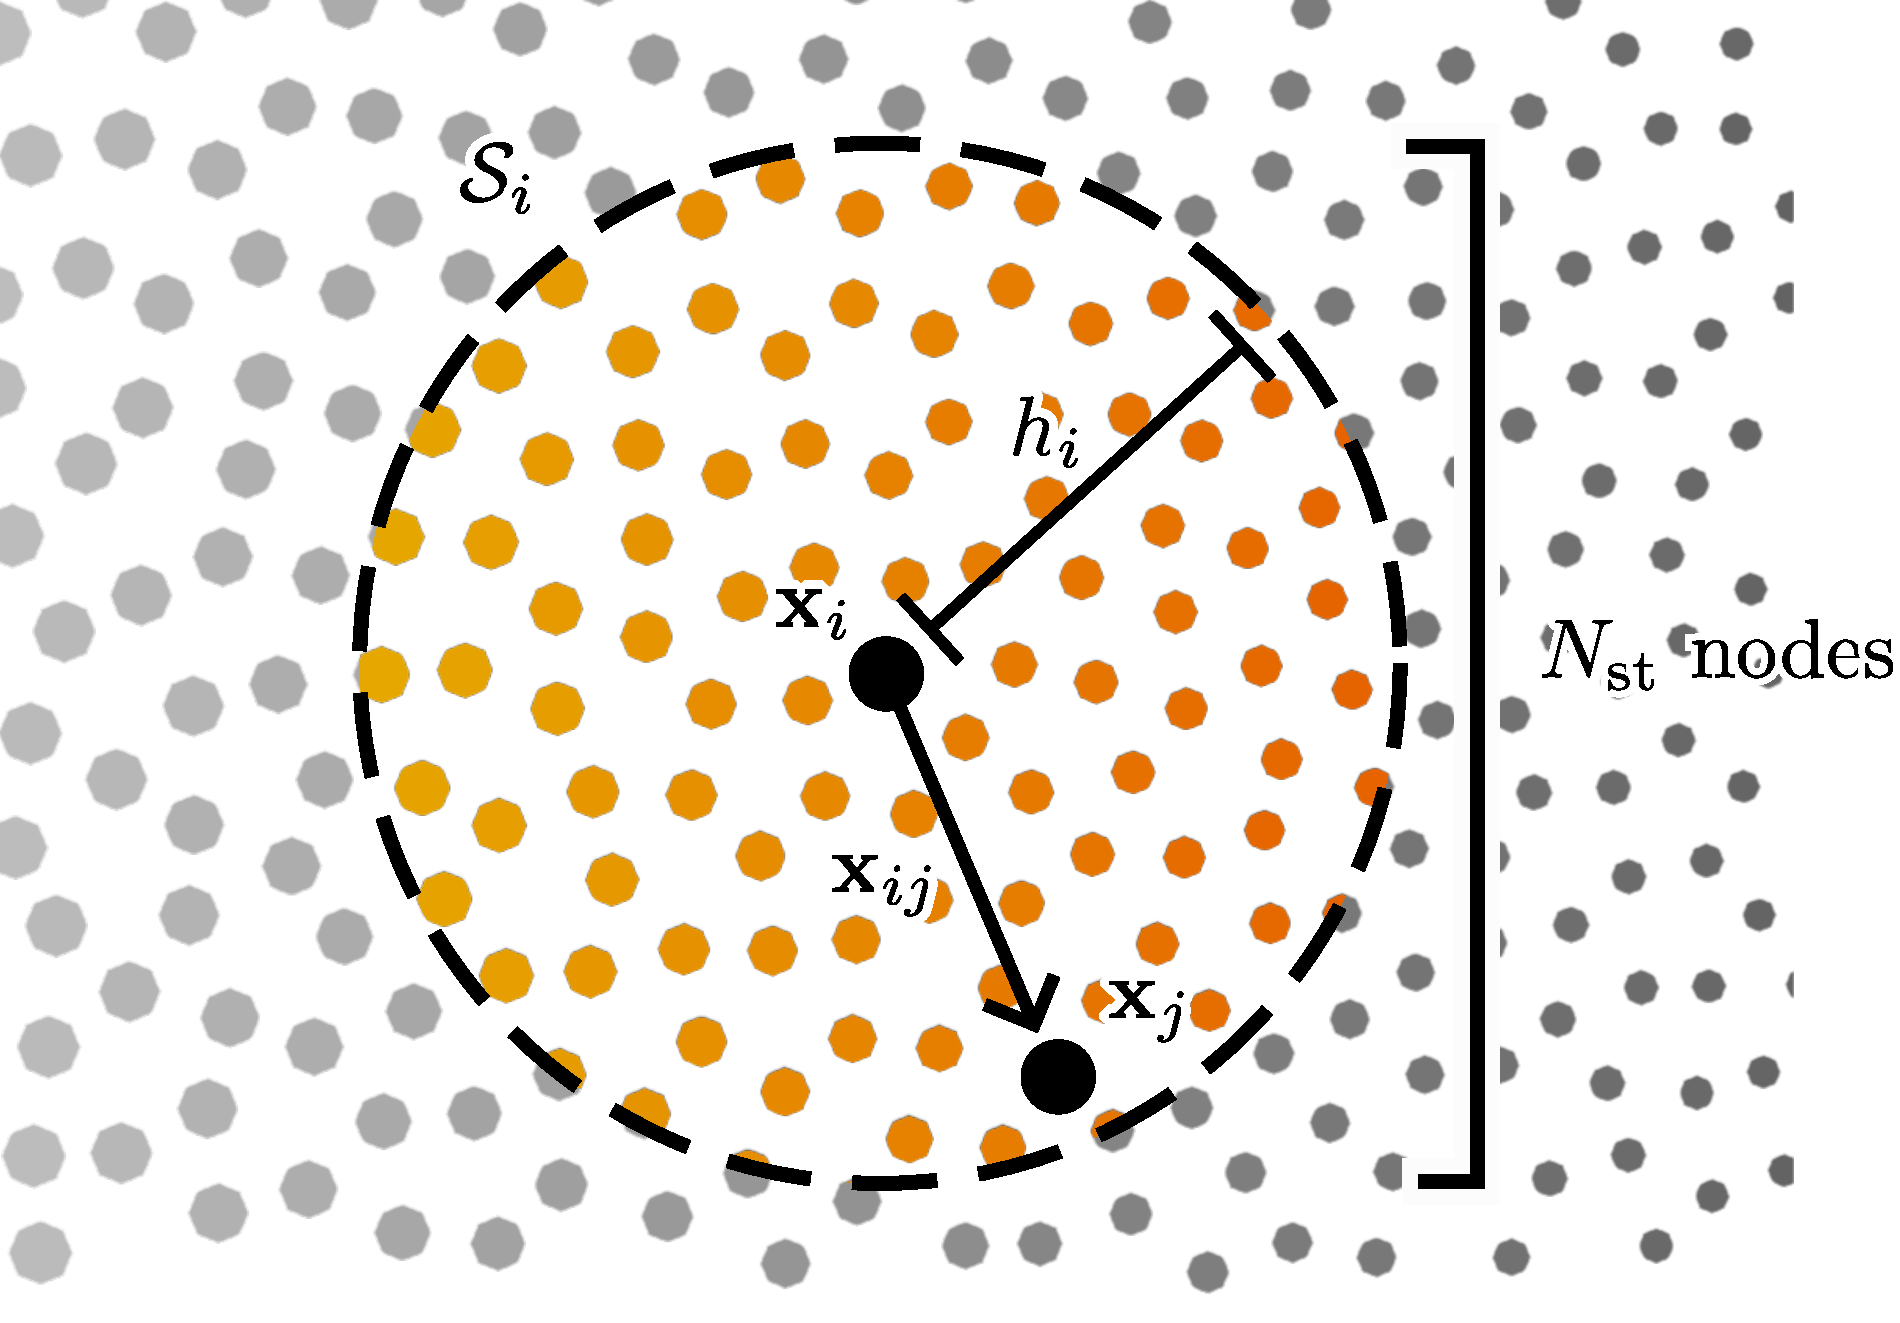
\includegraphics[scale=0.175]{assets/imgs/labfm-stencil-drawn_simple.pdf}
\caption{CAPTION}
\label{fig:labfm-stencil}
\end{figure}
        
    